% ======================================================================
% JPM Defense Deck (Beamer) — Factor Volatility Asymmetry: GARCH vs EGARCH
% 30-min mixed audience (PMs / Risk / Academics)
% ======================================================================

\documentclass[aspectratio=169,10pt]{beamer}

% -------------------- Theme / Style --------------------
\usetheme{Madrid}
\usecolortheme{dolphin}
\setbeamertemplate{navigation symbols}{}
\setbeamertemplate{footline}[frame number]

\usepackage[utf8]{inputenc}
\usepackage[T1]{fontenc}
\usepackage[english]{babel}

\usepackage{amsmath, amsfonts, amssymb}
\usepackage{graphicx}
\usepackage{booktabs}
\usepackage{tabularx}
\usepackage{threeparttable}
\usepackage{siunitx}
\usepackage{hyperref}
\usepackage{xcolor}

% -------------------- Graphics --------------------
% Put all images next to this .tex or in ./figures/
% and keep these filenames:
% 02_cum_returns.png
% 03_corr_full.png
% 05_vol_overlay.png
% 10_var_backtest_spx.png
% 11_news_impact_curves.png
% 12b_regime_return_distributions.png
% 12_vol_regime_analysis.png
% 13_persistence_halflife_leverage.png
% 14_garch_efficient_frontier.png
\graphicspath{{./}{./figures/}}

% -------------------- Metadata --------------------
\title[Asymmetric Factor Volatility]{Asymmetric Factor Volatility and Tail Risk:\\ GARCH vs EGARCH in U.S. Equity Factors}
\subtitle{Evidence from U.S. equity factors}
\author{Youssef Louraoui}
\institute{\quad (youssef.louraoui@essec.edu)}
\date{\today}

% -------------------- Helpers --------------------
\newcommand{\imp}{\textbf{Key implication:} }
\newcommand{\kpi}[1]{\textbf{\color{blue}#1}}
\newcommand{\warn}[1]{\textbf{\color{red}#1}}

% ======================================================================
\begin{document}

% -------------------- Title --------------------
\begin{frame}
  \titlepage
\end{frame}

% -------------------- Agenda --------------------
\begin{frame}{Agenda}
\small
\begin{enumerate}
  \item \kpi{A-1. Motivation \& stakes:} why factor volatility misspecification matters
  \item \kpi{B-2. Data \& design:} factors, regimes, models, evaluation
  \item \kpi{D-3. Core results:} asymmetry, persistence, VaR backtests, regimes
  \item \kpi{C-4. Portfolio implications:} correlation convergence \& conditional frontier
  \item \kpi{E-5. Conclusion:} what changes for PMs / risk, limitations, extensions
\end{enumerate}
% \vspace{4pt}
% % \imp Minimal math in main deck; full equations and tests in Appendix.
\end{frame}

% ======================================================================
% A-1 Motivation
% ======================================================================
\section{A-1 Motivation \& Impact}

\begin{frame}{A-1 | The risk problem: why factor volatility modeling matters}
\small
\begin{itemize}
  \item Risk systems rely on volatility forecasts for \textbf{position sizing, VaR, margin, hedging timing}.
  \item Standard symmetric GARCH assumes: \emph{positive and negative shocks of same magnitude} $\Rightarrow$ \emph{same vol response}.
  \begin{itemize}
    \item \kpi{Non-normal returns:} fat tails + negative skew across factors
    \item \kpi{Asymmetric volatility transmission:} ``bad news'' increases volatility more than ``good news''
  \end{itemize}
\end{itemize}

\vspace{6pt}
\begin{block}{Practical consequence}
\warn{Underestimating volatility in crisis peaks} can delay hedging and understate tail risk precisely when correlation rises and diversification collapses.
\end{block}
\end{frame}

\begin{frame}{A-1 | Executive summary}
\small
\begin{enumerate}
  \item \kpi{Asymmetry is universal:} EGARCH leverage $\gamma < 0$ for all factors (2014--2026).
  \item \kpi{Tail risk calibration improves:} EGARCH reduces VaR exceedances vs GARCH (SPX example).
  \item \kpi{Regimes matter:} risk-adjusted performance varies materially by volatility regime.
  \item \kpi{Diversification is state-dependent:} correlations are structurally high; rise further in stress.
  \item \kpi{Portfolio optimization shifts:} conditional covariance pushes min-var into defensive concentration.
\end{enumerate}
\end{frame}

% ======================================================================
% B-2 Data & Design
% ======================================================================
\section{B-2 Data \& Empirical Design}

\begin{frame}{B-2 | Data universe}
\small
\begin{columns}[T,onlytextwidth]
\column{0.58\textwidth}
\begin{itemize}
  \item Daily returns, 2014--2026
  \item \kpi{Market:} SPX proxy (SPY)
  \item \kpi{Style factors (ETFs as proxies):}
  \begin{itemize}
    \item Momentum (MTUM)
    \item Value (VLUE)
    \item Quality (QUAL)
    \item Minimum Volatility (USMV)
    \item Size (IWM)
  \end{itemize}
  \item Focus: conditional volatility, asymmetry, tail risk, and allocation implications.
\end{itemize}

\column{0.42\textwidth}
\begin{block}{Deliverable}
A volatility-and-regime aware framework that tells a PM/risk team:
\begin{itemize}
  \item when symmetric models break,
  \item how tail metrics react,
  \item how allocation set compresses.
\end{itemize}
\end{block}
\end{columns}
\end{frame}

\begin{frame}{B-2 | Visual context: factor performance over the full sample}
\centering

\includegraphics[width=0.8\textwidth]{02_cum_returns.png}
\vspace{2pt}

\small
\only<1>{\imp Cumulative behavior differs, but risk is driven by \emph{time-varying volatility} and \emph{time-varying dependence}.}
\only<2>{\imp Next: show dependence is \emph{structurally high} (not orthogonal premia).}
\end{frame}

\begin{frame}{B-2 | Dependence: unconditional correlations are already high}
\centering
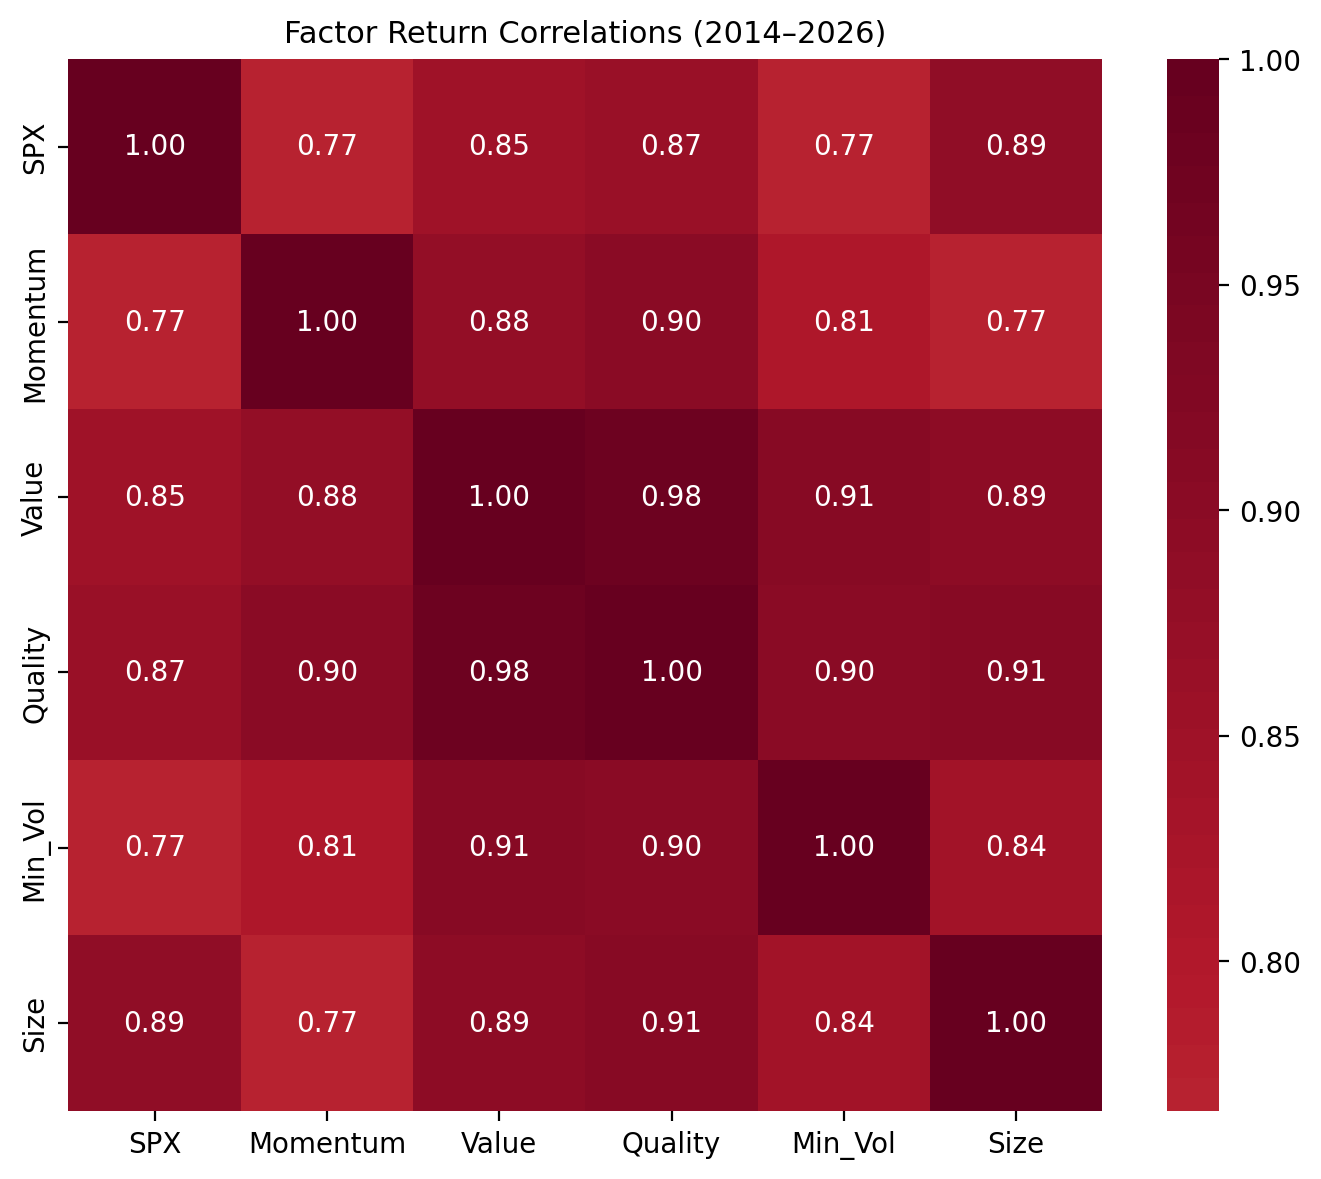
\includegraphics[width=0.4\textwidth]{03_corr_full.png}

\small
\begin{itemize}
\item Correlations are uniformly high (roughly 0.77 to 0.98 in your heatmap).
\item \imp Multi-factor diversification is \textbf{weaker than textbook intuition} even before conditioning on regimes.
\end{itemize}
\end{frame}

\begin{frame}{B-2 | Model set (kept simple in main deck)}
\small
\begin{columns}[T,onlytextwidth]
\column{0.52\textwidth}
\begin{block}{Symmetric baseline}
GARCH(1,1): volatility reacts to squared shocks symmetrically.
\end{block}

\column{0.48\textwidth}
\begin{block}{Asymmetric extension}
EGARCH(1,1): log-variance + leverage term.
\vspace{2pt}

\imp The \textbf{sign} of shocks matters: negative returns can increase future volatility more.
\end{block}
\end{columns}

% \vspace{6pt}
% \only<1>{
% \begin{itemize}
%   \item Main deck: intuition + empirical evidence.
%   \item Appendix: full equations, Kupiec test, stationarity notes.
% \end{itemize}
% }
\end{frame}

% ======================================================================
% D-3 Core Results
% ======================================================================
\section{D-3 Core Results (Vol, Asymmetry, Tail Risk, Regimes)}

\begin{frame}{D-3 | Conditional volatility: GARCH vs EGARCH (all factors)}
\centering

\includegraphics[width=0.45\textwidth]{05_vol_overlay.png}

\small
\only<1>{\imp Both models cluster volatility; differences are largest around crisis spikes.}
\only<2>{\imp EGARCH tracks downside-driven volatility surges more aggressively (consistent with leverage/asymmetry).}
\end{frame}

\begin{frame}{D-3 | Asymmetry: news impact curves (leverage effect)}
\centering

\includegraphics[width=0.5\textwidth]{11_news_impact_curves.png}

\small
\begin{itemize}
  \item In your estimates, \kpi{$\gamma<0$ across all series} $\Rightarrow$ bad news increases volatility more than good news.
  \item \imp Even defensive sleeves (Quality, MinVol) show material asymmetry.
\end{itemize}
\end{frame}

\begin{frame}{D-3 | Persistence, half-life, leverage (summary)}
\centering

\includegraphics[width=0.8\textwidth]{13_persistence_halflife_leverage.png}

\small
\only<1>{
\begin{itemize}
  \item GARCH persistence near unity implies shocks decay over \textbf{weeks}.
  \item \imp Regimes are sticky enough to matter for allocation and risk budgeting.
\end{itemize}
}
\only<2>{
\begin{itemize}
  \item \kpi{Leverage ranking:} Value/Quality strongest (largest negative $\gamma$), SPX weakest.
  \item \imp Style factors can amplify downside volatility transmission vs the broad market.
\end{itemize}
}
\end{frame}

\begin{frame}{D-3 | Tail risk calibration: SPX 99\% VaR backtest}
\centering

\includegraphics[width=0.8\textwidth]{10_var_backtest_spx.png}

\small
\begin{itemize}
  \item Visual: exceedances cluster in stress.
  \item \imp EGARCH reduces exceedances vs GARCH in your SPX backtest, but extreme tails still challenge Gaussian GARCH-class models.
\end{itemize}
\end{frame}

\begin{frame}{D-3 | Regime logic: volatility states \& distributional shifts}
\centering

\includegraphics[width=0.7\textwidth]{12b_regime_return_distributions.png}

\small
\only<1>{\imp High-vol regimes show fatter tails across factors (distributional deterioration in stress).}
\only<2>{\imp This is where tail metrics and diversification assumptions break simultaneously.}
\end{frame}

\begin{frame}{D-3 | Regime counts + conditional Sharpe proxy (portfolio-relevant)}
\centering
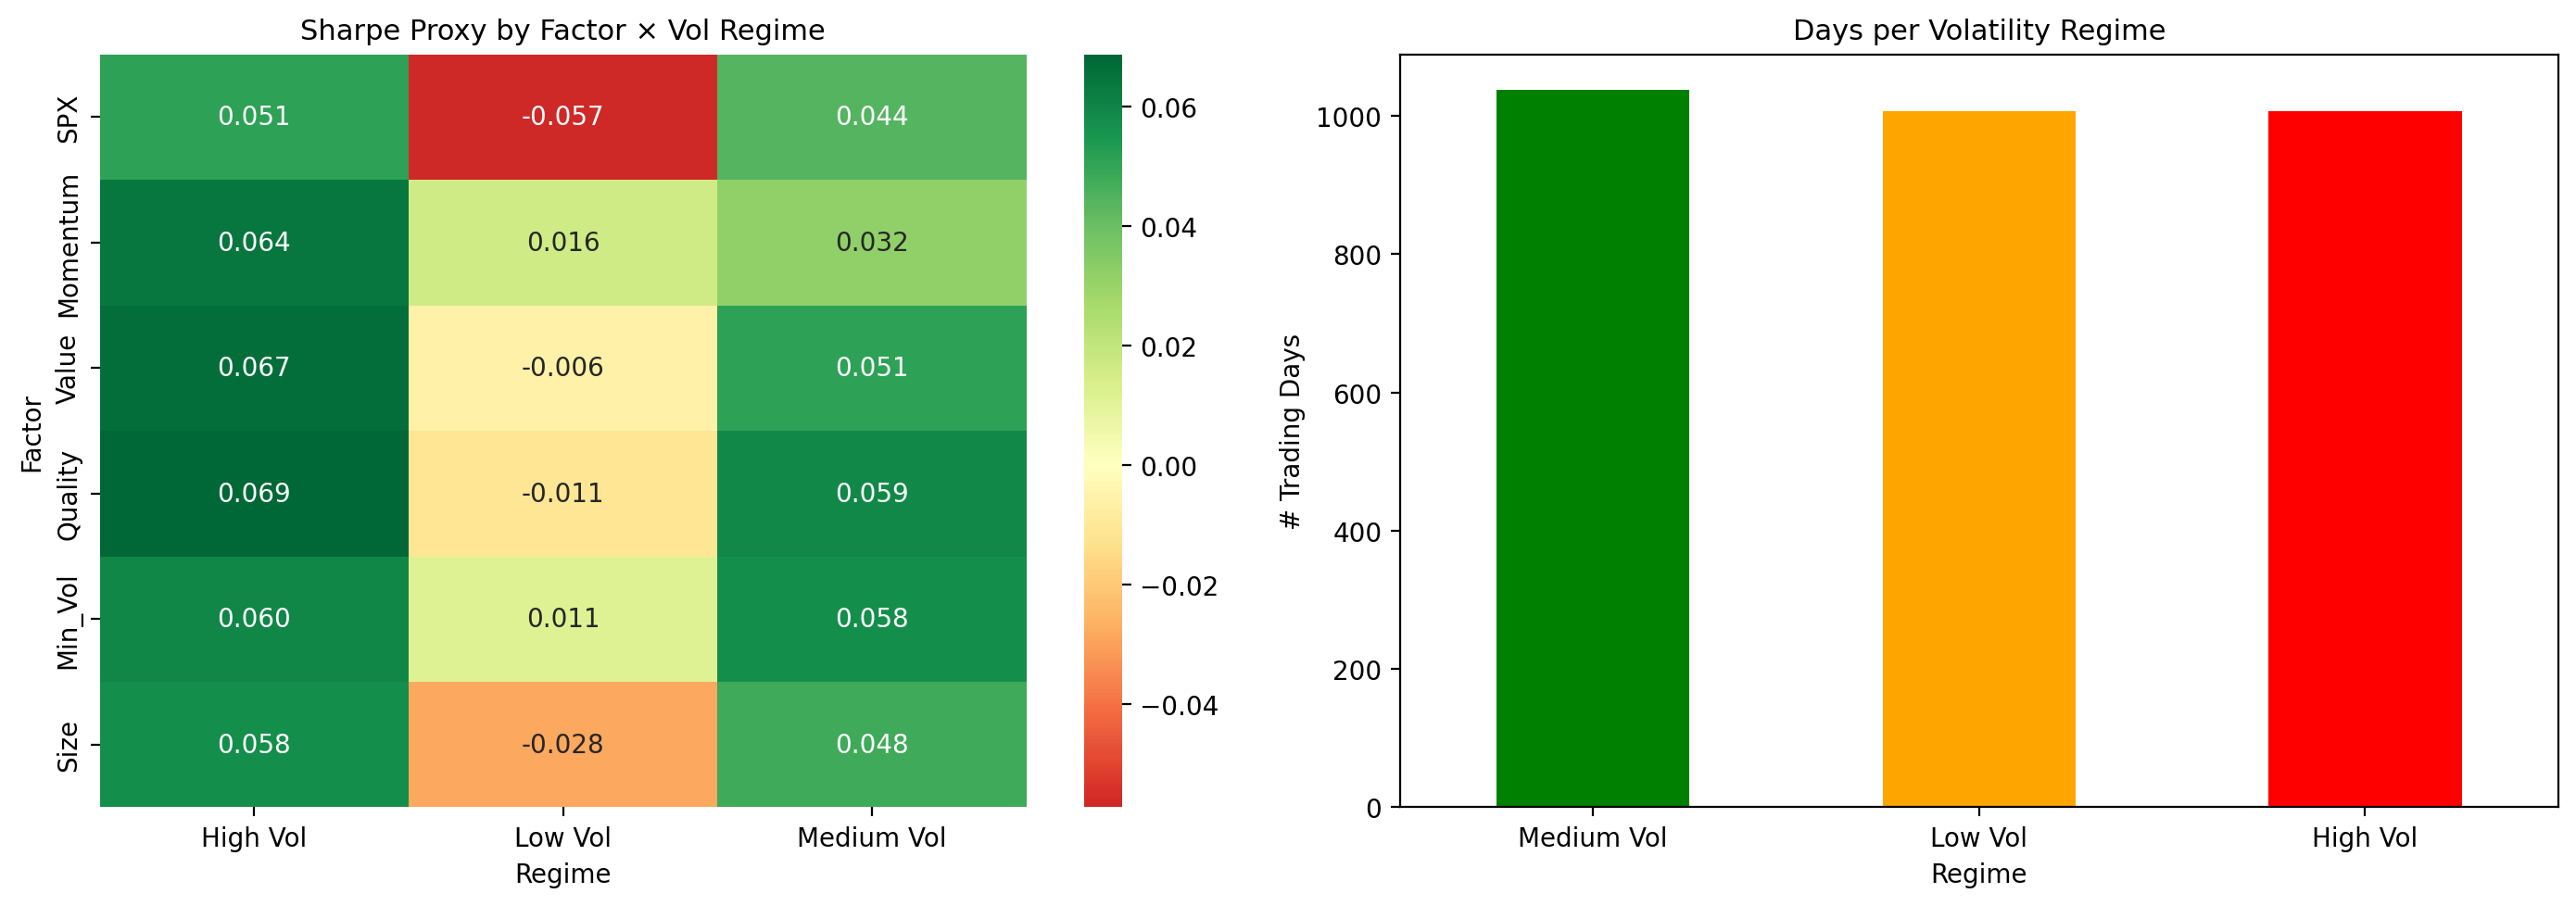
\includegraphics[width=0.75\textwidth]{12_vol_regime_analysis.png}

\small
\begin{itemize}
  \item \kpi{Risk-adjusted performance is state-dependent}.
  \item \imp Low-vol is not automatically the best regime for Sharpe-proxy across all sleeves.
\end{itemize}
\end{frame}

% ======================================================================
% C-4 Portfolio Implications
% ======================================================================
\section{C-4 Portfolio Construction Implications}

\begin{frame}{C-4 | Mechanism: why diversification collapses in stress}
\small
\begin{columns}[T,onlytextwidth]
\column{0.56\textwidth}
\begin{block}{Three forces jointly}
\begin{enumerate}
  \item \kpi{Volatility persistence} (shocks last weeks)
  \item \kpi{Leverage effect} ($\gamma<0$; downside amplifies vol)
  \item \kpi{Correlation convergence} (already high; rises in stress)
\end{enumerate}
\end{block}

\column{0.44\textwidth}
\begin{block}{Portfolio-level outcome}
\begin{itemize}
  \item Conditional covariance tightens
  \item Efficient frontier compresses
  \item Min-var can degenerate to defensive concentration
\end{itemize}
\end{block}
\end{columns}
\end{frame}

\begin{frame}{C-4 | Conditional frontier (GARCH-based covariance snapshot)}
\centering

\includegraphics[width=0.7\textwidth]{14_garch_efficient_frontier.png}

\small
\only<1>{\imp Equal weight is not neutral under heteroskedasticity; it becomes an implicit risk bet.}
\only<2>{\imp Min-variance concentrates in MinVol in your results: a live example of ``diversification collapse'' in a highly correlated factor set.}
\end{frame}

\begin{frame}{C-4 | What changes for PMs and Risk? (actionable)}
\small
\begin{block}{Implementation-level guidance}
\begin{itemize}
  \item \kpi{Model choice should be regime-aware:} symmetric models can be fragile in downside shocks.
  \item \kpi{Tail calibration at 99\% is the hard problem:} 95\% can look fine while 99\% fails.
  \item \kpi{Stress-time correlation is the hidden driver:} factor diversification can vanish when you need it.
  \item \kpi{Allocation should use conditional covariance:} volatility parity / defensive scaling can be a robust baseline vs naive min-var or equal weight.
\end{itemize}
\end{block}

\only<2>{
\begin{block}{Key takeaway}
This is not “EGARCH is always better.” It is:
\textbf{model asymmetry + regimes + dependence} $\Rightarrow$ \textbf{better risk calibration and allocation behavior when it matters}.
\end{block}
}
\end{frame}

% ======================================================================
% E-5 Conclusion
% ======================================================================
\section{E-5 Conclusion, Limits, Extensions}

\begin{frame}{E-5 | Conclusions}
\small
\begin{enumerate}
  \item \kpi{Universal leverage effect:} all factors show $\gamma<0$ (bad news raises vol more).
  \item \kpi{Tail risk is systematically underestimated in stress:} EGARCH improves but does not fully solve 99\% tails.
  \item \kpi{Regime dependence is economically meaningful:} volatility states persist long enough to guide risk budgeting.
  \item \kpi{Diversification is state-dependent:} high structural correlations imply limited orthogonality among sleeves.
  \item \kpi{Portfolio implication:} conditional covariance can force defensive concentration; risk parity is a pragmatic middle ground.
\end{enumerate}
\end{frame}

\begin{frame}{E-5 | Limitations}
\small
\begin{itemize}
  \item Gaussian innovations: extreme tails may require \kpi{Student-$t$}, EVT overlays, or filtered historical simulation.
  \item Univariate modeling: dependence is treated largely via correlations and a conditional covariance snapshot; a next step is \kpi{multivariate DCC / asymmetric GARCH}.
  \item ETF proxies: factor implementation details (index methodology, rebalancing, transaction costs) can matter.
\end{itemize}

\begin{block}{Key takeaway on limitations}
Even with conservative modeling choices, the data still delivers the same core story:
\textbf{asymmetry + persistence + high dependence} $\Rightarrow$ \textbf{fragile tail risk and compressed frontier in stress}.
\end{block}
\end{frame}

\begin{frame}{E-5 | Extensions}
\small
\begin{columns}[T,onlytextwidth]
\column{0.52\textwidth}
\begin{block}{Risk-model extensions}
\begin{itemize}
  \item EGARCH with Student-$t$ innovations
  \item EVT overlay on standardized residuals
  \item CoVaR / systemic tail measures (multi-sleeve)
\end{itemize}
\end{block}

\column{0.48\textwidth}
\begin{block}{Allocation extensions}
\begin{itemize}
  \item Dynamic volatility targeting by sleeve
  \item Regime-conditioned covariance + stress overlays
  \item Robust optimization under correlation spikes
\end{itemize}
\end{block}
\end{columns}
\end{frame}

% ======================================================================
% Appendix
% ======================================================================
\appendix
\section*{Appendix}

\begin{frame}{Appendix | Model equations}
\small
\begin{block}{GARCH(1,1)}
\[
\sigma_t^2 = \omega + \alpha \varepsilon_{t-1}^2 + \beta \sigma_{t-1}^2
\]
\end{block}

\begin{block}{EGARCH(1,1)}
\[
\ln(\sigma_t^2) = \omega + \beta \ln(\sigma_{t-1}^2)
+ \alpha \left(\frac{|\varepsilon_{t-1}|}{\sigma_{t-1}} - \mathbb{E}|z|\right)
+ \gamma \frac{\varepsilon_{t-1}}{\sigma_{t-1}}
\]
\end{block}

\imp Interpretation: $\gamma<0$ means downside shocks drive disproportionately higher future volatility.
\end{frame}

\begin{frame}{Appendix | Kupiec POF test (unconditional coverage)}
\small
\begin{block}{Kupiec (1995) likelihood ratio}
\[
LR_{\mathrm{POF}} = -2 \ln
\left(
\frac{(1-\alpha)^{N-x} \alpha^x}
{(1-\hat{p})^{N-x} \hat{p}^x}
\right)
\]
\end{block}

\begin{itemize}
  \item $N$ = number of VaR forecasts, $x$ = number of exceedances, $\alpha$ = nominal tail prob.
  \item Under correct coverage, $LR_{\mathrm{POF}} \sim \chi^2(1)$ asymptotically.
\end{itemize}
\end{frame}

\begin{frame}{Appendix | References}
\small
\begin{thebibliography}{99}
\bibitem{engle1982} Engle (1982), Econometrica.
\bibitem{bollerslev1986} Bollerslev (1986), Journal of Econometrics.
\bibitem{nelson1991} Nelson (1991), Econometrica.
\bibitem{engleng1993} Engle \& Ng (1993), Journal of Finance.
\bibitem{kupiec1995} Kupiec (1995), Journal of Derivatives.
\bibitem{longin2001} Longin \& Solnik (2001), Journal of Finance.
\bibitem{angchen2002} Ang \& Chen (2002), Journal of Financial Economics.
\bibitem{markowitz1952} Markowitz (1952), Journal of Finance.
\end{thebibliography}
\end{frame}

\begin{frame}{Extensive list of references}

\begin{thebibliography}{99}

\bibitem{adrian2016} Adrian, T., and M. K. Brunnermeier. “CoVaR.” American Economic Review, 106 (2016), pp. 1705–1741.

\bibitem{ang2013} Ang, A. “Factor Investing.” SSRN Electronic Journal (2013), pp. 1–72.

\bibitem{ang2002} Ang, A., and G. Bekaert. “International Asset Allocation with Regime Shifts.” Review of Financial Studies, 15 (2002), pp. 1137–1187.

\bibitem{angchen2002} Ang, A., and J. Chen. “Asymmetric Correlations of Equity Portfolios.” Journal of Financial Economics, 63 (2002), pp. 443–494.

\bibitem{ang2006} Ang, A., R. J. Hodrick, Y. Xing, and X. Zhang. “The Cross-Section of Volatility and Expected Returns.” Journal of Finance, 61 (2006), pp. 259–299.

\bibitem{asness2018} Asness, C. S., and L. H. Pedersen. “Quality Minus Junk.” Review of Accounting Studies (2018).

\bibitem{barroso2015} Barroso, P., and P. Santa-Clara. “Momentum Has Its Moments.” Journal of Financial Economics, 116 (2015), pp. 111–120.

\bibitem{bernankes1999} Bernanke, B. S., M. Gertler, and S. Gilchrist. “The Financial Accelerator in a Quantitative Business Cycle Framework.” Handbook of Macroeconomics, 1 (1999), pp. 1341–1393.

\bibitem{black1976} Black, F. “Studies of Stock Price Volatility Changes.” Proceedings of the American Statistical Association, Business and Economic Statistics Section (1976), pp. 177–181.

\bibitem{blitz2020} Blitz, D., M. Hanauer, and M. Vidojevic. “The Idiosyncratic Momentum Anomaly.” International Review of Economics and Finance, 69 (2020).

\bibitem{bollerslev1986} Bollerslev, T. “Generalized Autoregressive Conditional Heteroskedasticity.” Journal of Econometrics, 31 (1986), pp. 307–327.

\bibitem{campbell1992} Campbell, J. Y., and L. Hentschel. “No News Is Good News: An Asymmetric Model of Changing Volatility in Stock Returns.” Journal of Financial Economics, 31 (1992), pp. 281–318.

\bibitem{carhart1997} Carhart, M. “On Persistence in Mutual Fund Performance.” Journal of Finance, 52 (1997), pp. 57–82.

\bibitem{christie1982} Christie, A. A. “The Stochastic Behavior of Common Stock Variances: Value, Leverage and Interest Rate Effects.” Journal of Financial Economics, 10 (1982), pp. 407–432.

\bibitem{christoffersen1998} Christoffersen, P. F. “Evaluating Interval Forecasts.” International Economic Review, 39 (1998), pp. 841–862.

\bibitem{daniel2016} Daniel, K., and T. J. Moskowitz. “Momentum Crashes.” Journal of Financial Economics, 122 (2016), pp. 221–247.

\bibitem{ding1993} Ding, Z., C. W. J. Granger, and R. F. Engle. “A Long Memory Property of Stock Market Returns and a New Model.” Journal of Empirical Finance, 1 (1993), pp. 83–106.

\bibitem{engle1982} Engle, R. F. “Autoregressive Conditional Heteroscedasticity with Estimates of the Variance of United Kingdom Inflation.” Econometrica, 50 (1982), pp. 987–1007.

\bibitem{engle1993} Engle, R. F., and V. K. Ng. “Measuring and Testing the Impact of News on Volatility.” Journal of Finance, 48 (1993), pp. 1749–1778.

\bibitem{fama1993} Fama, E. F., and K. R. French. “Common Risk Factors in the Returns on Stocks and Bonds.” Journal of Financial Economics, 33 (1993), pp. 3–56.

\bibitem{fama2015} Fama, E. F., and K. R. French. “A Five-Factor Asset Pricing Model.” Journal of Financial Economics, 116 (2015), pp. 1–22.

\bibitem{ferson1991} Ferson, W. E., and C. R. Harvey. “The Variation of Economic Risk Premiums.” Journal of Political Economy, 99 (1991), pp. 385–415.

\bibitem{foglia2021} Foglia, M. “Smart Beta Allocation and Macroeconomic Variables: The Impact of COVID-19.” MDPI (2021).

\bibitem{forbes2022} Forbes, K. J. and Rigobon, R. “No Contagion, Only Interdependence: Measuring Stock Market Comovements” Journal of Finance, 57-5 (2022), pp. 2223-2261.

\bibitem{frazzini2014} Frazzini, A., and L. H. Pedersen. “Betting Against Beta.” Journal of Financial Economics, 111 (2014), pp. 1–25.

\bibitem{grossman1980} Grossman, S., and J. Stiglitz. “On the Impossibility of Informationally Efficient Markets.” American Economic Review, 70 (1980), pp. 393–408.

\bibitem{hasaj2021} Hasaj, M., and B. Sherer. “COVID-19 and Smart-Beta: A Case Study on the Role of Sectors.” EDHEC-Risk Institute Working Paper (2021).

\bibitem{jegadeesh1993} Jegadeesh, N., and S. Titman. “Returns to Buying Winners and Selling Losers.” Journal of Finance, 48 (1993), pp. 65–91.

\bibitem{jensen1967} Jensen, M. C. “The Performance of Mutual Funds in the Period 1945–1964.” Journal of Finance, 23 (1967), pp. 389–416.

\bibitem{kupiec1995} Kupiec, P. H. “Techniques for Verifying the Accuracy of Risk Measurement Models.” Journal of Derivatives, 3 (1995), pp. 73–84.

\bibitem{longin2001} Longin, F., and B. Solnik. “Extreme Correlation of International Equity Markets.” Journal of Finance, 56 (2001), pp. 649–676.

\bibitem{malkiel2014} Malkiel, B. G. “Is Smart Beta Really Smart?” Journal of Portfolio Management, 40 (2014), pp. 127–134.

\bibitem{mangram2013} Mangram, M. E. “A Simplified Perspective of the Markowitz Portfolio Theory.” SSRN Electronic Journal (2013).

\bibitem{markowitz1952} Markowitz, H. “Portfolio Selection.” Journal of Finance, 7 (1952), pp. 77–91.

\bibitem{nelson1991} Nelson, D. B. “Conditional Heteroskedasticity in Asset Returns: A New Approach.” Econometrica, 59 (1991), pp. 347–370.

\bibitem{novymarx2016} Novy-Marx, R., and M. Velikov. “A Taxonomy of Anomalies and Their Trading Costs.” Review of Financial Studies, 29 (2016), pp. 104–147.

\bibitem{pagano2020} Pagano, M., C. Wagner, and J. Zechner. “Disaster Resilience and Asset Prices.” SSRN Electronic Journal (2020).

\bibitem{sharpe1964} Sharpe, W. F. “Capital Asset Prices: A Theory of Market Equilibrium under Conditions of Risk.” Journal of Finance, 19 (1964), pp. 425–442.

\bibitem{sharpe1991} Sharpe, W. F. “Capital Asset Prices with and without Negative Holdings.” Journal of Finance, 46 (1991), pp. 489–509.

\end{thebibliography}
\end{frame}

\end{document}